\documentclass[tikz]{standalone}

\usetikzlibrary{positioning}

\begin{document}
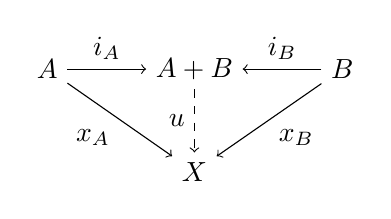
\begin{tikzpicture}
	\node (A) {$A$};
	\node [right=1.0cm of A] (Q) {$A+B$};
	\node [right=1.0cm of Q] (B) {$B$};
	\node [below=0.8cm of Q] (X) {$X$};
	\draw [->] (A) to node [above] {$i_A$} (Q);
	\draw [->] (B) to node [above] {$i_B$} (Q);
	\draw [->, dashed] (Q) to node [left] {$u$} (X);
	\draw [->] (A) to node [below left] {$x_A$} (X);
	\draw [->] (B) to node [below right] {$x_B$} (X);
\end{tikzpicture}
\end{document}
